\chapter{ChIP-seq as a High-Throughoutput Sequencing Technique}
%\todo{ChIP-seq je spíš metoda než technologie}

\section{Considerations of Experimental Design}

\begin{figure}[b!]
    \centering
    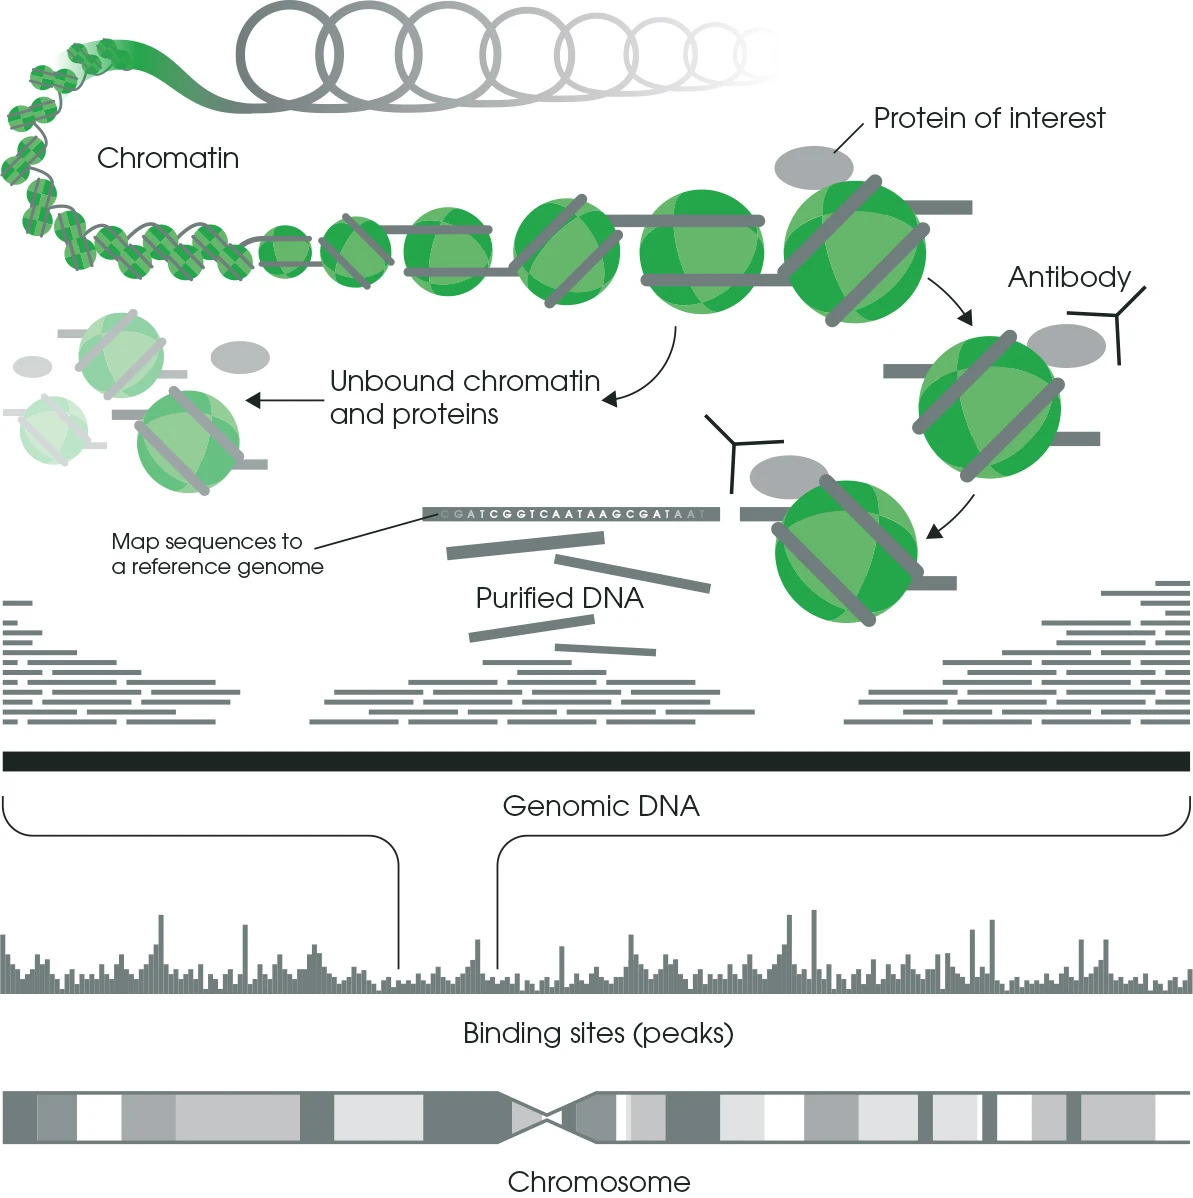
\includegraphics[width=\textwidth]{../img/chip.jpeg}
    \captionsource{Overview of ChIP-seq experiment.}{www.abcam.com}
    \label{fig:graph_classes}
\end{figure}

A typical ChIP-seq protocol has many steps and requires a sufficient quantity of immunoenriched DNA. 
The consideration of the first step depends on the properties of the protein under investigation. 
For example, histone-DNA interactions are strong enough. 
Thus the fixation using formaldehyde as a crosslinking agent may not be necessary~\cite{barski2008identification}. 
On the other hand, proteins associated with DNA for a short time require a crosslinking step. 
In the case of histone deacetylases (HDACs) and histone acetyltransferases (HATs), an additional disuccinimidyl glutarate (DSG) treatment step before formaldehyde crosslinking is required to preserve protein-protein associations~\cite{wang2009genome}. 


Cross-linked chromatin is fragmented before ChIP. 
The way of the fragmentation depends on the purpose of the experiment, cell type, number of cells, fixation conditions. 
For nucleosome modifications, MNase digestion may be preferred~\cite{kidder2011chip}.  
The method allows generating high-resolution data of mononucleosome sized particles. 
However, the nucleosome instability may cause the loss of signal.
To identify TF binding events, sonication of crosslinked chromatin is a preferable method. 
In this case, the micrococcal nuclease may cause degradation of the linker DNA~\cite{kidder2011chip}.
The sonication conditions should be optimized for each experiment type. 
A sonication buffer can influence the result~\cite{steger2008dot1l}. 
It is also important to avoid oversonication during the library preparation for transcription factors. 
Oversonication may lead to the destruction of protein epitopes in cross-linked chromatin~\cite{ostrow2015chip}. 




The successful ChIP experiment depends on the isolation of the protein under study from a complex mixture of the chromatin fragments and associated proteins. 
The target protein bound to the chromatin can be isolated from a sample using an antibody pre-immobilized onto insoluble magnetic beads that specifically recognizes that protein and that purification technique is known as immunoprecipitation (IP). 
After incubation, the immune complexes are separated from the lysate of non-interacting DNA by applying a magnetic field~\cite{slovakova2005use}.

The right choice of antibody is an essential factor for the ChIP-seq experiment. 
Many experiments focus on newly discovered proteins, which means that such a protein probably does not have any available antibody. 
However, the development and validation of the antibodies to each protein is very time-consuming and expensive~\cite{jarvik1998epitope}. 
For example, the number of proteins interacting with chromatin in a human cell is very high~\cite{ramani2005consolidating}, and the traditional approach may not be suitable.
Genetic engineering makes it possible to solve that problem by fusion of a short epitope sequence into a gene of interest for which an antibody is available~\cite{jarvik1998epitope,brizzard2008epitope,goldberg2010distinct}. 
This recombinant DNA method is called epitope tagging and was first described in 1984~\cite{munro1984use}. 





\section{Library Construction and Sequencing}

After chromatin purification with and without immunoprecipitation to prepare ChIP and corresponding input DNA fragments, DNA fragments undergo the library construction by ligation of adapters, which are designed to interact with the NGS platform.


The size range of $150$ to $300$ bp fragment length selection is equivalent to mono- and dinucleosome chromatin fragments~\cite{kidder2011chip}.

With the invention of the thermal cycler,  Sanger chain-termination sequencing method, which is referred to as first-generation sequencing (FGS), enables automatization of the sequencing process~\cite{quail2012tale}. 
The appearance of the pyrosequencing technique was the start of the next-generation sequencers (NGS). 
Unlike Sanger's sequencing, this method enabled real-time observation; and usage of nucleotides, which are not heavily modified~\cite{ronaghi1996real, ronaghi1998sequencing}.
Instead, the method uses luminescent labeling for measuring of pyrophosphate production. 
First, ATP sulfurylase converts pyrophosphate into ATP. 
The ATP is used as a substrate for the luciferase enzyme, which catalyzes a light-emitting reaction. 
The light produced by the enzyme can be measured and is proportional to the amount of pyrophosphate. 
The measuring of the pyrophosphate produced during the reaction is used to identify the sequence~\cite{hyman1988new}. 
Like Sanger's, such a method is called sequencing by synthesis (SBS).

\paragraph{Sequencing by synthesis.}
Solexa/Illumina\textsuperscript{\texttrademark} platform is the most common SBS method today~\cite{voelkerding2009next}. 
The bridge amplification produces clusters of clonal DNA. 
Fluorescent reversible-terminator (RT) nucleotides cannot bind further nucleotides due to protection at $3^\prime$ hydroxyl position~\cite{heather2016sequence}. 
During sequencing, free RT nucleotides are able, in a competitive manner, to  be incorporated into the nascent DNA chain based on complimentarity to the DNA template, following the removal of the fluorescent tag, which is different for four bases and can be imaged by an analyzer~\cite{berglund2011next}. 
Illumina\textsuperscript{\texttrademark} HiSeq and MiSeq machine enable us to reach greater read length and depth. 
However, the recent NextSeq 500 technology reduces capturing time and cost by replacing the four-channel sequencing system with a two-channel system~\cite{reuter2015high}. 



The goal of the ChIP-sequencing is to obtain reads long enough to map uniquely to the reference. 
Multiple barcoded ChIP-seq libraries can be pooled together and sequenced in a single lane~\cite{craig2008identification} to reduce the cost of the experiment and produce high-quality data.
In many cases, 36-50 bp will be enough even for a complex organism such as a human. 
The longer the reads sequenced, and/or the higher the number of reads, the deeper coverage per base may be achieved.
The main advantage of the Illumina\textsuperscript{\texttrademark} platform is the ability to obtain paired-end sequenced data. 
Paired-end sequencing generates high sequencing coverage, improves alignment efficiency into repetitive regions, detects fragment size, and increases the probability of the alignment to a reference~\cite{kidder2011chip, chen2012systematic}.



\paragraph{Semiconductor sequencing.}
Another remarkable sequencing platform called IonTorrent\textsuperscript{\texttrademark} is also available on the market. 
Instead of using laser scanners, IonTorrent\textsuperscript{\texttrademark} technology measures pH during the sequencing without using labeled nucleotides. 
However, the homopolymeric regions may cause errors due to electronic signals corresponding to the number of released hydrogen ions~\cite{ambardar2016high}.
To improve the sequencing indel error rates and reduce GC-bias the technology comes up with a sequencing enzyme called Hi-Q~\cite{veras2014efficiency}. 










\section{ChIP-seq Read Mapping to the Reference}

\paragraph{Raw data.}
Raw data of short sequenced tags often appear in FASTQ format containing sequence information and quality scores, and may often contain 10s to 100s million reads.
In FASTQ files each entry is associated with 4 lines:


\begin{verbatim}
@SEQ_ID
GATTTGGGGTTCAAAGCAGTATCGATCAAATAGTAAATCCATTTGTTCAACTCACAGTTT
+
!''*((((***+))%%%++)(%%%%).1***-+*''))**55CCF>>>>>>CCCCCCC65
\end{verbatim}

First line contains sequence identifier and additional information.
Second line contains a short read in standard nucleotide code.
Third line always begins with '+' character.
And the last line encodes quality value for the short read from the second line.


\paragraph{Alignment.}
The sequence information from FASTQ files should be reconstructed by the alignment to the reference genome and finding overlaps.
Several alignment tools have been developed based on extended Burrows-Wheeler transform (BWT). 
The algorithm was developed in 1994 as a data compression technique~\cite{li2009fast, siren2014indexing}.
And at the end of the 2000s was applied in the NGS field~\cite{simpson2010efficient}.
Suitable tools~\cite{langmead2009ultrafast, li2009fast, kim2019graph} map sequenced reads producing  SAM (Sequence Alignment Map), BAM (Binary Alignment Map), or relatively new CRAM output. 
BAM format is a widely used standard so far.

Many mapping software tools can search for exon junctions. 
However, unlike RNA-seq, the ChIP-seq experiment does not require to find spliced alignment.
Thus the optimal setting of the parameters is to disable the spliced alignment and minimize the number of the allowed mismatches, increasing the number of the unique mapped reads and simplify further analysis~\cite{derrien2012fast}.

\paragraph{Mismatches.}
Alignment mismatches can be observed due to the biological differences between the genotype of the analyzed organism (indels and SNPs) and the reference genome~\cite{park2009chip}.
It is also possible to observe differences between reference and mapped tags due to contamination by the adapters or primers, which can be computationally filtered when their sequence is known~\cite{nakamura2011sequence}. 
Sequencing platforms may also produce sequence-specific errors (SSE). 
Some of them may be avoided or minimized by the improvement of the experimental procedure. 
The latest experiments tend to increase the number of sequencing cycles up to 150 bp. 
During the sequencing of the longer reads on the Illumina\textsuperscript{\texttrademark} platform, errors are more likely to be produced~\cite{nakamura2011sequence}.

\paragraph{Mapping sensitivity.}
Some sequences are able to fit more than one location in the reference. Thus, allowing the random site for multiple mapped reads may increase the sensitivity of peak detection. 
The ratio of the unique mapped reads over the total number of mapped reads is one of the parameters of the library quality assessment and should not be below 50\%~\cite{shin2013computational}.













%%%%%%%%%%%%%%%%%%%%%%%%%%%%%%%%%%%%%%%%%%%%%%%%%%%%%%%%%%%%%%%
\section{Quality control and computational analysis workflow}


ChIP-seq data analysis is a powerful tool to get new insight into transcription control machinery and other biological processes. 
However, computational pipelines have not been straightforward; 
and new tools and analysis pipelines are needed to be developed.

NCBI's SRA and GEO~\cite{barrett2012ncbi} are the largest central public domains containing a vast amount of published genomic data, including ChIP-seq datasets. 
Many algorithms and tools have been introduced for addressing specific aspects of computational analysis. 
As was mentioned above, raw data often appear in FASTQ format. 
Processing pipelines are developed to make raw sequence reads annotated.
Low-quality data can be filtered before alignment to the reference. 
But such filtering is not necessary due to the inability of such sequences to be aligned~\cite{furey2012chip}.


\paragraph{Quality problems.}
Data quality problem is one of the most critical ChIP-seq experiment issues due to artifacts and noise reproducibility.
In a typical TF study reads mapped to the same genomic coordinate are filtered as redundant, because the expected number of mapped reads per genomic position is less than or equal to one. 
%% \todo{až teď mi došlo, že tenhle kousek vlastně nechápu "the expected number of mapped reads per base pair is less than 1."}
On the other hand, highly repetitive regions such as rDNA, long repetitive elements such as segmental duplication regions are the regions linked to important biological functions~\cite{nakato2017recent}. But the annotation of such regions is challenging and requires special algorithms that take such regions into account~\cite{chung2011discovering}.

\paragraph{Quality metrics.}
Data processing routine requires quality control at an early step, reducing further downstream analysis problems~\cite{ewels2016multiqc}.
To obtain reliable results, it is essential to have a complex ChIP-seq library.
The complexity is measured by the non-redundant fraction (NRF), which is one of the QC-metrics.
The fraction is defined as the ratio between uniquely mapped reads over the total number of reads~\cite{landt2012chip}.

Other quality metrics that can be used to assess a ChIP sample are normalized cross-correlation (NSC) and relative cross-correlation (RSC) metrics of the fragment length and read length~\cite{landt2012chip, marinov2014large}. 
The directionality of the sequencing reads produces bimodal enrichment on both strands centered around the binding site of the protein of interest. 
The cross-correlation metric can evaluate each obtained peak. 
The calculation is based on Pearson's linear correlation between forward and reverse strand for each complementary base by shifting the minus strand. 
The procedure generates two peaks, a bigger one corresponding to the fragment length, and a smaller one is associated with a read length. 



%%%%%%%%%%%%%%%%%%%%%%%%%%%%%%%%%%%%%%%%%%%%%%%%%%%%%%%%%%%
\section{The best strategy}
\label{strategy}

Extracting useful information from huge data repositories combines techniques from computer science and statistics~\cite{friedman2001elements}. 
%\todo{místo "lore" bych použil "information" nebo "knowledge".}
In terms of ChIP-seq, the main goal is to distinguish significant enrichment events from background noise and to compare multiple profiles that are linked to the biological functions. 
The process of discovering patterns in large datasets is critically dependent on high data quality. 
Cell culture conditions, incubation, ChIP, and library construction may cause variability between datasets. 
To identify true ChIP signals the availability of at least two biological replicates is necessary~\cite{kidder2011chip}. 
The availability of two or more replicates helps to assess whether the signal is a true biological event or just a random variation. 

The ChIP-seq experiment should be consistent. 
Candidate peak regions should have a similar signal profile, and that consistency is measured by the percentage of the overlapping peaks, correlation coefficient over selected intervals, and Irreproducible Discovery rate (IDR)~\cite{shin2013computational}.

For proper binding site detection, the fragmented chromatin is divided into two portions. 
One portion undergoes all the immunoprecipitation procedure described above, whereas the other is sequenced directly. 
This is referred to as an input control dataset and used to normalize IP sequencing results~\cite{kidder2011chip}. 
Another control dataset can be generated using IP protocol, with an irrelevant antibody $-$ mock IP~\cite{flensburg2014comparison}. 
Both controls are informative and have advantages as well as disadvantages.
The choice of the right control dataset will be described more in detail in section~\ref{control}.
%\todo{popiš konkrétní vyhody a nevýhody těchto dvou typů kontrol, anebo odkaž čtenáře na kapitolu, kde to popisuješ}

In addition to both input and mock normalization methods, there is also spike-in normalization, in which foreign chromatin is used as internal control and helps avoid several biases~\cite{bonhoure2014quantifying}.
Spike-based signal adjustment allows comparing the occupancy levels. 
By adding a constant low amount of foreign chromatin to samples before immunoprecipitation, the method can help detect global changes in occupancy. 